% answers.tex —— 2016 年·全国Ⅱ卷·文科 · 参考答案与详细解析片段
% 由 tools/generate_projects.py 依来源总账自 2016/2016_数学真题_全国2文_试题.md + 2016/2016_数学真题_全国2文_解析正文.md + 2016/2016_数学真题_全国2文_答案要点.md 生成，勿手改（改源 MD 后重跑）


\begin{gktip}
以下解析由本项目依据固定原卷独立推导，并经另一角色盲核（D），非官方解析。原卷第 18 题重复标注“(2)”的两项在此均保留原编号。
\end{gktip}

\gkpart{选择题}

\begin{answer}
\gksolhead{1}{}

\textbf{题目}：

已知集合 $A=\{1,2,3\}$，$B=\{x\mid x^2<9\}$，则 $A\cap B=$（　）

   (A) $\{-2,-1,0,1,2,3\}$　(B) $\{-2,-1,0,1,2\}$　(C) $\{1,2,3\}$　(D) $\{1,2\}$

\Needspace{4\baselineskip}
\textbf{解析}

由 $x^2<9$ 得 $-3<x<3$，所以 $B$ 中的整数为 $-2,-1,0,1,2$。与 $A=\{1,2,3\}$ 取交集时，$3$ 不满足严格不等式。

\gkanswer{答案：D，\(\{1,2\}\)}

\end{answer}
\begin{answer}
\gksolhead{2}{}

\textbf{题目}：

设复数 $z$ 满足 $z+i=3-i$，则 $z=$（　）

   (A) $-1+2i$　(B) $1-2i$　(C) $3+2i$　(D) $3-2i$

\Needspace{4\baselineskip}
\textbf{解析}

由 $z+i=3-i$，得 $z=3-2i$，与题面所求一致。

\gkanswer{答案：D，\(3-2\mathrm i\)}

\end{answer}
\begin{answer}
\gksolhead{3}{}

\textbf{题目}：

函数 $y=A\sin(\omega x+\varphi)$ 的部分图象如图所示，则（　）
\nopagebreak[4]
\begin{center}% 2016 年全国卷Ⅱ文科第 3 题：正弦函数局部图象
\begin{tikzpicture}[>=Stealth, line width=0.45pt]
  \draw[->] (-0.92,0) -- (1.72,0) node[right] {$x$};
  \draw[->] (0,-2.62) -- (0,2.42) node[above] {$y$};

  \draw[dashed] (0,2) -- ({pi/3},2);
  \draw[dashed] ({pi/3},0) -- ({pi/3},2);
  \draw[dashed] ({-pi/6},0) -- ({-pi/6},-2);

  \draw[line width=0.8pt, domain=-0.72:1.30, samples=100, smooth, variable=\x]
    plot ({\x},{2*sin(deg(2*\x-pi/6))});

  \node[left=1pt] at (0,2) {$2$};
  \node[right=1pt] at (0,-2) {$-2$};
  \node[anchor=north east] at ({-pi/6},-0.04) {$-\dfrac{\pi}{6}$};
  \node[below=2pt] at ({pi/3},0) {$\dfrac{\pi}{3}$};
  \node[below left=1pt] at (0,0) {$O$};
\end{tikzpicture}
\end{center}
\nopagebreak[4]
   (A) $y=2\sin\left(2x-\dfrac{\pi}{6}\right)$　(B) $y=2\sin\left(2x-\dfrac{\pi}{3}\right)$

   (C) $y=2\sin\left(x+\dfrac{\pi}{6}\right)$　(D) $y=2\sin\left(x+\dfrac{\pi}{3}\right)$

\Needspace{4\baselineskip}
\textbf{解析}

图象振幅为 $2$。从极小值点 $x=-\frac{\pi}{6}$ 到极大值点 $x=\frac{\pi}{3}$ 的距离为 $\frac{\pi}{2}$，是半个周期，所以周期 $T=\pi$、角频率 $\omega=2$。代入极大值点可确定相位，得到对应的正弦函数。

\gkanswer{答案：A，\(y=2\sin(2x-\frac{\pi}{6})\)}

\end{answer}
\begin{answer}
\gksolhead{4}{}

\textbf{题目}：

体积为 $8$ 的正方体的顶点都在同一球面上，则该球面的表面积为（　）

   (A) $12\pi$　(B) $\dfrac{32}{3}\pi$　(C) $8\pi$　(D) $4\pi$

\Needspace{4\baselineskip}
\textbf{解析}

正方体棱长为 $\sqrt[3]{8}=2$，体对角线长为 $2\sqrt3$，外接球半径为 $\sqrt3$。球面面积为 $4\pi(\sqrt3)^2$。

\gkanswer{答案：A，\(12\pi\)}

\end{answer}
\begin{answer}
\gksolhead{5}{}

\textbf{题目}：

设 $F$ 为抛物线 $C:y^2=4x$ 的焦点，曲线 $y=\dfrac{k}{x}\ (k>0)$ 与 $C$ 交于点 $P$，$PF\perp x$，则 $k=$（　）

   (A) $\dfrac12$　(B) $1$　(C) $\dfrac32$　(D) $2$

\Needspace{4\baselineskip}
\textbf{解析}

抛物线 $y^2=4x$ 的焦点为 $F=(1,0)$。由 $PF\perp x$ 轴，点 $P$ 的横坐标为 $1$；代入抛物线得纵坐标为 $\pm2$。又 $P$ 在 $y=\frac{k}{x}$ 上且 $k>0$，故 $y_P=k>0$，取正纵坐标即得 $k=2$。

\gkanswer{答案：D，\(2\)}

\end{answer}
\begin{answer}
\gksolhead{6}{}

\textbf{题目}：

圆 $x^2+y^2-2x-8y+13=0$ 的圆心到直线 $ax+y-1=0$ 的距离为 $1$，则 $a=$（　）

   (A) $-\dfrac43$　(B) $-\dfrac34$　(C) $\sqrt3$　(D) $2$

\Needspace{4\baselineskip}
\textbf{解析}

\Needspace{5\baselineskip}
配方得圆心 $(1,4)$、半径 $2$。圆心到直线 $ax+y-1=0$ 的距离满足
\nopagebreak[4]
\[
\frac{|a+3|}{\sqrt{a^2+1}}=1.
\]
平方后得 $(a+3)^2=a^2+1$，解得 $a=-\frac43$。

\gkanswer{答案：A，\(-\frac43\)}

\end{answer}
\begin{answer}
\gksolhead{7}{}

\textbf{题目}：

如图是由圆柱与圆锥组合而成的几何体的三视图，则该几何体的表面积为（　）
\nopagebreak[4]
\begin{center}% 2016 年全国卷Ⅱ文科第 7 题：圆柱与圆锥组合几何体的三视图
\begin{tikzpicture}[>=Stealth, scale=0.9, line width=0.45pt, font=\small]
  % 两幅立面图：圆柱矩形与圆锥三角形共用底边。
  \draw (0,0) rectangle (2,2);
  \draw (0,2) -- (1,{2+sqrt(3)}) -- (2,2);
  \draw (3,0) rectangle (5,2);
  \draw (3,2) -- (4,{2+sqrt(3)}) -- (5,2);

  % 第一幅立面左侧的高度尺寸。
  \draw (-0.06,0) -- (-0.38,0);
  \draw (-0.06,2) -- (-0.38,2);
  \draw[<->] (-0.38,0) -- (-0.38,2);
  \node[left=2pt] at (-0.38,1) {$4$};
  \draw (-0.06,{2+sqrt(3)}) -- (-0.38,{2+sqrt(3)});
  \draw[<->] (-0.38,2) -- (-0.38,{2+sqrt(3)});
  \node[left=2pt] at (-0.38,{2+sqrt(3)/2}) {$2\sqrt{3}$};

  % 两幅立面图下方的宽度尺寸。
  \draw (0,-0.06) -- (0,-0.36);
  \draw (2,-0.06) -- (2,-0.36);
  \draw[<->] (0,-0.36) -- (2,-0.36);
  \node[below=1pt] at (1,-0.36) {$4$};
  \draw (3,-0.06) -- (3,-0.36);
  \draw (5,-0.06) -- (5,-0.36);
  \draw[<->] (3,-0.36) -- (5,-0.36);
  \node[below=1pt] at (4,-0.36) {$4$};

  % 俯视图。
  \draw (1,-2.15) circle (1);
  \fill (1,-2.15) circle (1.2pt);
\end{tikzpicture}
\end{center}
\nopagebreak[4]
   (A) $20\pi$　(B) $24\pi$　(C) $28\pi$　(D) $32\pi$

\Needspace{4\baselineskip}
\textbf{解析}

\Needspace{5\baselineskip}
三视图给出圆柱底面半径 $2$、高 $4$；圆锥底面半径也是 $2$，高为 $2\sqrt3$，母线长为 $4$。外露表面积由圆柱侧面、圆锥侧面和圆柱下底面组成：
\nopagebreak[4]
\[
2\pi\cdot2\cdot4+\pi\cdot2\cdot4+\pi\cdot2^2=28\pi.
\]
圆柱与圆锥的接触圆面不计入外露面积。

\gkanswer{答案：C，\(28\pi\)}

\end{answer}
\begin{answer}
\gksolhead{8}{}

\textbf{题目}：

某路口人行横道的信号灯为红灯和绿灯交替出现，红灯持续时间为 $40$ 秒。若一名行人来到该路口遇到红灯，则至少需要等待 $15$ 秒才出现绿灯的概率为（　）

   (A) $\dfrac7{10}$　(B) $\dfrac58$　(C) $\dfrac38$　(D) $\dfrac3{10}$

\Needspace{4\baselineskip}
\textbf{解析}

遇到红灯后，剩余红灯时间在 $0$ 到 $40$ 秒间均匀分布。至少等待 $15$ 秒等价于剩余红灯时间不少于 $15$ 秒，可选时长为 $40-15=25$ 秒，所求概率为 $\frac{25}{40}$。

\gkanswer{答案：B，\(\frac58\)}

\end{answer}
\begin{answer}
\gksolhead{9}{}

\textbf{题目}：

中国古代有计算多项式值的秦九韶算法，如图是实现该算法的程序框图。执行该程序框图，若输入的 $x=2$，$n=2$，依次输入的 $a$ 为 $2,2,5$，则输出的 $s=$（　）
\nopagebreak[4]
\begin{center}% 2016 年全国卷Ⅱ文科第 9 题：秦九韶算法程序框图
\begin{tikzpicture}[>=Stealth, font=\small, line width=0.45pt,
  box/.style={draw, minimum width=2.45cm, minimum height=0.56cm, inner sep=2pt},
  io/.style={draw, trapezium, trapezium left angle=70, trapezium right angle=110,
             minimum width=2.45cm, minimum height=0.58cm, inner sep=2pt},
  term/.style={draw, rounded corners=5pt, minimum width=1.35cm, minimum height=0.48cm, inner sep=2pt},
  dec/.style={draw, diamond, aspect=3.1, minimum width=2.75cm, minimum height=0.72cm, inner sep=1pt}]
  \node[term] (start) at (0,0) {开始};
  \node[io] (input) at (0,-0.92) {输入 $x,n$};
  \node[box] (init) at (0,-1.92) {$k=0,\ s=0$};
  \node[io] (inputa) at (0,-2.95) {输入 $a$};
  \node[box, minimum width=2.65cm, minimum height=1.04cm, align=center] (step) at (0,-3.96)
    {$s=s\cdot x+a$\\$k=k+1$};
  \node[dec] (condition) at (0,-5.08) {$k>n$};
  \node[io] (output) at (0,-6.05) {输出 $s$};
  \node[term] (finish) at (0,-6.95) {结束};

  \draw[->] (start.south) -- (input.north);
  \draw[->] (input.south) -- (init.north);
  \draw[->] (init.south) -- (inputa.north);
  \draw[->] (inputa.south) -- (step.north);
  \draw[->] (step.south) -- (condition.north);
  \draw[->] (condition.south) -- node[right=2pt] {是} (output.north);
  \draw[->] (output.south) -- (finish.north);

  \draw (condition.east) -- (2.0,-5.08) -- (2.0,-2.53);
  \draw[->] (2.0,-2.53) -- (0,-2.53);
  \node[above=2pt] at (1.7,-5.08) {否};
\end{tikzpicture}
\end{center}
\nopagebreak[4]
   (A) $7$　(B) $12$　(C) $17$　(D) $34$

\Needspace{4\baselineskip}
\textbf{解析}

程序每轮执行 $s\leftarrow2s+a$。由初值 $s=0$ 开始，依次输入 $2,2,5$，得到 $2,6,17$。处理完三个系数后循环结束，输出最后的 $s$。

\gkanswer{答案：C，\(17\)}

\end{answer}
\begin{answer}
\gksolhead{10}{}

\textbf{题目}：

下列函数中，其定义域和值域分别与函数 $y=10^{\lg x}$ 的定义域和值域相同的是（　）

   (A) $y=x$　(B) $y=\lg x$　(C) $y=2^x$　(D) $y=\dfrac1{\sqrt{x}}$

\Needspace{4\baselineskip}
\textbf{解析}

$10^{\lg x}=x$ 的定义域和值域均为 $(0,+\infty)$。选项 D 的函数 $\frac1{\sqrt{x}}$ 同样要求 $x>0$，且值域也是全部正实数。

\gkanswer{答案：D，\(y=\frac1{\sqrt{x}}\)}

\end{answer}
\begin{answer}
\gksolhead{11}{}

\textbf{题目}：

函数 $f(x)=\cos 2x+6\cos\left(\dfrac\pi2-x\right)$ 的最大值为（　）

   (A) $4$　(B) $5$　(C) $6$　(D) $7$

\Needspace{4\baselineskip}
\textbf{解析}

\Needspace{5\baselineskip}
令 $u=\sin x\in[-1,1]$，则
\nopagebreak[4]
\[
f(x)=\cos2x+6\sin x=1-2u^2+6u.
\]
关于 $u$ 的导数为 $6-4u\ge2>0$，所以最大值在 $u=1$ 处取得，函数值为 $1-2+6=5$。

\gkanswer{答案：B，\(5\)}

\end{answer}
\begin{answer}
\gksolhead{12}{}

\textbf{题目}：

已知函数 $f(x)\ (x\in\mathbb R)$ 满足 $f(x)=f(2-x)$，若函数 $y=|x^2-2x-3|$ 与 $y=f(x)$ 图象的交点为 $(x_1,y_1),(x_2,y_2),\ldots,(x_m,y_m)$，则 $\displaystyle\sum_{i=1}^{m}x_i=$（　）

   (A) $0$　(B) $m$　(C) $2m$　(D) $4m$

\Needspace{4\baselineskip}
\textbf{解析}

由 $f(x)=f(2-x)$，函数 $y=f(x)$ 关于直线 $x=1$ 对称。又
$x^2-2x-3=(x-1)^2-4$，所以 $y=|x^2-2x-3|$ 也关于 $x=1$ 对称。有限交点的横坐标成关于 $1$ 的对；每对之和为 $2$，若有交点落在对称轴上，其横坐标为 $1$。因此全部 $m$ 个横坐标之和为 $m$。

\gkanswer{答案：B，\(m\)}

\end{answer}
\gkpart{填空题}

\begin{answer}
\gksolhead{13}{}

\textbf{题目}：

已知向量 $\boldsymbol a=(m,4)$，$\boldsymbol b=(3,-2)$，且 $\boldsymbol a\parallel\boldsymbol b$，则 $m=$\gkblank{}。

\Needspace{4\baselineskip}
\textbf{解析}

平行向量的行列式为零：
$m(-2)-4\cdot3=0$，解得 $m=-6$。

\gkanswer{答案：\(-6\)}

\end{answer}
\begin{answer}
\gksolhead{14}{}

\textbf{题目}：

\Needspace{5\baselineskip}
若 $x,y$ 满足约束条件
\nopagebreak[4]
\[
\begin{cases}
x-y+1\geqslant0,\\
x+y-3\geqslant0,\\
x-3\leqslant0,
\end{cases}
\]
则 $z=x-2y$ 的最小值为\gkblank{}。

\Needspace{4\baselineskip}
\textbf{解析}

约束边界围成的可行域顶点为 $(1,2),(3,0),(3,4)$。目标函数 $z=x-2y$ 在这些点的值依次为 $-3,3,-5$，最小值为 $-5$。

\gkanswer{答案：\(-5\)}

\end{answer}
\begin{answer}
\gksolhead{15}{}

\textbf{题目}：

$\triangle ABC$ 的内角 $A,B,C$ 的对边分别为 $a,b,c$，若 $\cos A=\dfrac45$，$\cos C=\dfrac5{13}$，$a=1$，则 $b=$\gkblank{}。

\Needspace{4\baselineskip}
\textbf{解析}

\Needspace{5\baselineskip}
由 $\cos A=\frac45$、$\cos C=\frac5{13}$，且 $A,C$ 为三角形内角，得 $\sin A=\frac35$、$\sin C=\frac{12}{13}$。又 $B=\pi-(A+C)$，故
\nopagebreak[4]
\[
\sin B=\sin(A+C)
=\frac35\cdot\frac5{13}+\frac45\cdot\frac{12}{13}
=\frac{63}{65}.
\]
由正弦定理及 $a=1$，有 $b=\frac{\sin B}{\sin A}=\frac{21}{13}$。

\gkanswer{答案：\(\frac{21}{13}\)}

\end{answer}
\begin{answer}
\gksolhead{16}{}

\textbf{题目}：

有三张卡片，分别写有 $1$ 和 $2$、$1$ 和 $3$、$2$ 和 $3$。甲、乙、丙三人各取走一张卡片，甲看了乙的卡片后说：“我与乙的卡片上相同的数字不是 $2$”；乙看了丙的卡片后说：“我与丙的卡片上相同的数字不是 $1$”；丙说：“我的卡片上的数字之和不是 $5$”，则甲的卡片上的数字是\gkblank{}。

\Needspace{4\baselineskip}
\textbf{解析}

丙的卡片数字和不是 $5$，故丙不可能持 $\{2,3\}$。乙与丙共有的数字不是 $1$，排除丙持 $\{1,3\}$ 的情况，因而丙持 $\{1,2\}$、乙持 $\{2,3\}$，甲持余下的 $\{1,3\}$。此时甲、乙共有数字 $3$，符合甲的陈述。

\gkanswer{答案：甲的卡片写有 \(1,3\)}

\end{answer}
\gkpart{解答题}

\begin{answer}
\gksolhead{17}{}

\textbf{题目}：

等差数列 $\{a_n\}$ 中，$a_3+a_4=4$，$a_5+a_7=6$。

   (1) 求 $\{a_n\}$ 的通项公式；

   (2) 设 $b_n=[a_n]$，求数列 $\{b_n\}$ 的前 $10$ 项和，其中 $[x]$ 表示不超过 $x$ 的最大整数，如 $[0.9]=0$，$[2.6]=2$。

\Needspace{4\baselineskip}
\textbf{解析}

\gksubpart{(1)}

\Needspace{5\baselineskip}
设等差数列首项为 $a_1$、公差为 $d$。由题设得
\nopagebreak[4]
\[
2a_1+5d=4,\qquad 2a_1+10d=6.
\]
相减得 $d=\frac25$，代回得 $a_1=1$，所以
$a_n=1+(n-1)\frac25=\frac{2n+3}{5}$。

\gksubpart{(2)}

前 $10$ 项的下取整依次为 $1,1,1,2,2,3,3,3,4,4$，求和得 $24$。

\gkanswer{答案（1）：\(a_n=\frac{2n+3}{5}\)}

\gkanswer{答案（2）：\(\sum_{n=1}^{10}b_n=24\)}

\end{answer}
\begin{answer}
\gksolhead{18}{}

\textbf{题目}：

某险种的基本保费为 $a$（单位：元），继续购买该险种的投保人称为续保人，续保人本年度的保费与其上年度出险次数的关联如下：

\begin{center}
\begin{tabular}{lrrrrrr}
\toprule
上年度出险次数 & 0 & 1 & 2 & 3 & 4 & $\geqslant5$ \\
\midrule
保费 & $0.85a$ & $a$ & $1.25a$ & $1.5a$ & $1.75a$ & $2a$ \\
\bottomrule
\end{tabular}
\end{center}

随机调查了该险种的 $200$ 名续保人在一年内的出险情况，得到如下统计表：

\begin{center}
\begin{tabular}{lrrrrrr}
\toprule
上年度出险次数 & 0 & 1 & 2 & 3 & 4 & $\geqslant5$ \\
\midrule
频数 & 60 & 50 & 30 & 30 & 20 & 10 \\
\bottomrule
\end{tabular}
\end{center}

(1) 记 $A$ 为事件：“一续保人本年度的保费不高于基本保费”。求 $P(A)$ 的估计值；

(2) 记 $B$ 为事件：“一续保人本年度的保费高于基本保费但不高于基本保费的 $160\%$”。求 $P(B)$ 的估计值；

(2) 求续保人本年度的平均保费估计值。

\Needspace{4\baselineskip}
\textbf{解析}

\gksubpart{(1)}

保费不高于基本保费对应上年度出险 $0$ 次或 $1$ 次，共 $60+50=110$ 人。以样本频率估计，$P(A)=\frac{110}{200}$。

\gksubpart{(2) 题面第一处编号}

保费高于 $a$ 且不高于 $1.6a$，对应上年度出险 $2$ 次或 $3$ 次，共 $30+30=60$ 人。因此 $P(B)=\frac{60}{200}$。

\gksubpart{(2) 原卷重复编号的末项}

\Needspace{5\baselineskip}
原卷紧接着再次以“(2)”编号要求平均保费估计值。按频数加权：
\nopagebreak[4]
\[
\frac{60(0.85a)+50a+30(1.25a)+30(1.5a)+20(1.75a)+10(2a)}{200}
=\frac{477}{400}a.
\]
$a$ 的单位为元，故平均保费结果的量纲也是元。答案要点将这两个按原卷顺序的结果放在同一个结构化“(2)”记录中，以避免重复小问 ID。

\gkanswer{答案（1）：\(P(A)=\frac{11}{20}\)}

\gkanswer{答案（2）：\(P(B)=\frac3{10}\)；原卷紧接着再次标作“(2)”的平均保费估计值为 \(\frac{477}{400}a\)}

\end{answer}
\begin{answer}
\gksolhead{19}{}

\textbf{题目}：

如图，菱形 $ABCD$ 的对角线 $AC$ 与 $BD$ 交于点 $O$，点 $E,F$ 分别在 $AD,CD$ 上，$AE=CF$，$EF$ 交 $BD$ 于点 $H$，将 $\triangle DEF$ 沿 $EF$ 折到 $\triangle D'EF$ 的位置。
\nopagebreak[4]
\begin{center}% 2016 年全国卷Ⅱ文科第 19 题：菱形与折叠后的五棱锥示意图
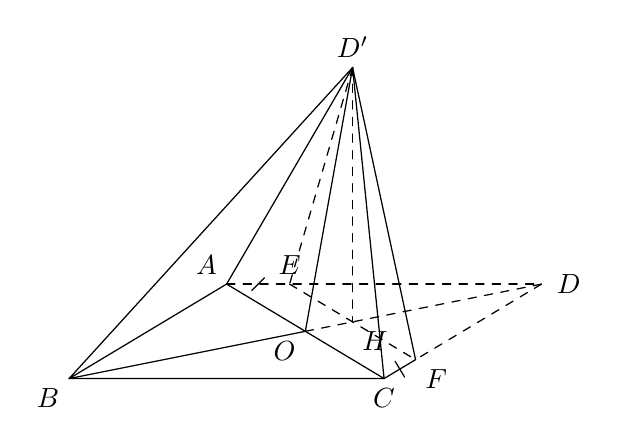
\begin{tikzpicture}[line width=0.45pt, line cap=round, line join=round]
  \coordinate (A) at (0,1.2);
  \coordinate (B) at (-2,0);
  \coordinate (C) at (2,0);
  \coordinate (D) at (4,1.2);
  \coordinate (O) at (1,0.6);
  \coordinate (E) at (0.8,1.2);
  \coordinate (F) at (2.4,0.24);
  \coordinate (H) at (1.6,0.72);
  \coordinate (Dp) at (1.6,3.95);

  % 菱形的后侧边及被遮挡的底面线段。
  \draw[dashed] (A) -- (D);
  \draw[dashed] (D) -- (F);
  \draw[dashed] (E) -- (H) -- (F);
  \draw[dashed] (O) -- (H) -- (D);

  % 菱形前侧边、对角线 AC 及可见的 BD 段。
  \draw (A) -- (B) -- (C) -- (F);
  \draw (A) -- (O) -- (C);
  \draw (B) -- (O);

  % 折起顶点 D' 与图中可见的棱、辅助连线。
  \draw (Dp) -- (A);
  \draw (Dp) -- (B);
  \draw[dashed] (Dp) -- (E);
  \draw (Dp) -- (O);
  \draw[dashed] (Dp) -- (H);
  \draw (Dp) -- (C);
  \draw (Dp) -- (F);

  % AE=CF 的等长记号。
  \draw (0.32,1.12) -- (0.48,1.28);
  \draw (2.14,0.22) -- (2.26,0.02);

  \node[above] at (Dp) {$D'$};
  \node[above left] at (A) {$A$};
  \node[below left] at (B) {$B$};
  \node[below] at (C) {$C$};
  \node[right=2pt] at (D) {$D$};
  \node[above] at (E) {$E$};
  \node[below right] at (F) {$F$};
  \node[below left] at (O) {$O$};
  \node[below right] at (H) {$H$};
\end{tikzpicture}
\end{center}
\nopagebreak[4]
   (1) 证明：$AC\perp HD'$；

   (2) 若 $AB=5$，$AC=6$，$AE=\dfrac54$，$OD'=2\sqrt2$，求五棱锥 $D'-ABCFE$ 的体积。

\Needspace{4\baselineskip}
\textbf{解析}

\gksubpart{(1)}

在菱形中 $AD=CD$，且 $AE=CF$，所以 $DE=DF$，从而
$\frac{DE}{DA}=\frac{DF}{DC}$，得到 $EF\parallel AC$。点 $H$ 在 $BD$ 上，而菱形对角线互相垂直，因此 $DH\perp AC$，也有 $DH\perp EF$。沿 $EF$ 折叠时 $H$ 固定，向量 $HD$ 绕与 $AC$ 平行的轴旋转为 $HD'$；垂直于旋转轴的向量旋转后仍垂直于该轴，故 $HD'\perp AC$。

\gksubpart{(2)}

取底面坐标 $O=(0,0)$、$A=(3,0)$、$C=(-3,0)$、$B=(0,4)$、$D=(0,-4)$。菱形边长为 $5$、对角线 $AC=6$。由 $AE=CF=\frac54$，得 $E=(\frac94,-1)$、$F=(-\frac94,-1)$，所以 $H=(0,-1)$，且 $HD=3$。

\Needspace{5\baselineskip}
菱形面积为 $\frac{6\cdot8}{2}=24$。三角形 $DEF$ 的底 $EF=\frac92$，高为 $3$，面积为 $\frac{27}{4}$，故五边形 $ABCFE$ 的面积为 $24-\frac{27}{4}=\frac{69}{4}$。令折叠后 $D'=(0,y,z)$；由折叠保长和 $OD'=2\sqrt2$ 得
\nopagebreak[4]
\[
(y+1)^2+z^2=9,\qquad y^2+z^2=8.
\]
\Needspace{5\baselineskip}
相减得 $y=0$，进而 $z^2=8$，棱锥高为 $2\sqrt2$。所以
\nopagebreak[4]
\[
V=\frac13\cdot\frac{69}{4}\cdot2\sqrt2=\frac{23\sqrt2}{2}.
\]

\gkanswer{答案（1）：\(AC\perp HD'\)}

\gkanswer{答案（2）：\(V_{D'-ABCFE}=\frac{23\sqrt2}{2}\)}

\end{answer}
\begin{answer}
\gksolhead{20}{}

\textbf{题目}：

已知函数 $f(x)=(x+1)\ln x-a(x-1)$。

   (1) 当 $a=4$ 时，求曲线 $y=f(x)$ 在点 $(1,f(1))$ 处的切线方程；

   (2) 若当 $x\in(1,+\infty)$ 时，$f(x)>0$，求 $a$ 的取值范围。

\Needspace{4\baselineskip}
\textbf{解析}

\gksubpart{(1)}

\Needspace{5\baselineskip}
当 $a=4$ 时，$f(1)=0$，并且
\nopagebreak[4]
\[
f'(x)=\ln x+1+\frac1x-a,\qquad f'(1)=-2.
\]
所以点 $(1,0)$ 处切线斜率为 $-2$。

\gksubpart{(2)}

\Needspace{5\baselineskip}
对 $x>1$，不等式条件化为
\nopagebreak[4]
\[
a<g(x):=\frac{(x+1)\ln x}{x-1}.
\]
\Needspace{5\baselineskip}
有 $\lim_{x\to1^+}g(x)=2$。又对 $x>1$，
\nopagebreak[4]
\[
\frac{d}{dx}\left(\ln x-\frac{2(x-1)}{x+1}\right)
=\frac{(x-1)^2}{x(x+1)^2}>0.
\]
括号内的式子在 $x=1$ 为 $0$，所以 $g(x)>2$。因此所有有限的 $x>1$ 均满足条件当且仅当 $a\le2$：若 $a=2$，仍有 $g(x)>2$；若 $a>2$，由极限可取充分接近 $1$ 的 $x$ 使 $g(x)<a$。

\gkanswer{答案（1）：切线方程 \(y=-2x+2\)}

\gkanswer{答案（2）：\(a\in(-\infty,2]\)}

\end{answer}
\begin{answer}
\gksolhead{21}{}

\textbf{题目}：

已知点 $A$ 是椭圆 $E:\dfrac{x^2}{4}+\dfrac{y^2}{3}=1$ 的左顶点，斜率为 $k\ (k>0)$ 的直线交椭圆 $E$ 于 $A,M$ 两点，点 $N$ 在 $E$ 上，$MA\perp NA$。

   (1) 当 $|AM|=|AN|$ 时，求三角形 $AMN$ 的面积；

   (2) 当 $2|AM|=|AN|$ 时，证明：$\sqrt3<k<2$。

\Needspace{4\baselineskip}
\textbf{解析}

设 $A=(-2,0)$。沿斜率 $k>0$ 的方向令 $M=A+s(1,k)$。代入椭圆方程得非零交点参数
\Needspace{5\baselineskip}
$s=\frac{12}{3+4k^2}$，故
\nopagebreak[4]
\[
|AM|=\frac{12\sqrt{1+k^2}}{3+4k^2}.
\]
\Needspace{5\baselineskip}
取垂直方向 $(-k,1)$，令 $N=A+v(-k,1)$，代入椭圆并取异于 $A$ 的交点，得 $v=-\frac{12k}{3k^2+4}$，所以
\nopagebreak[4]
\[
|AN|=\frac{12k\sqrt{1+k^2}}{3k^2+4}.
\]

\gksubpart{(1)}

\Needspace{5\baselineskip}
令两线段长度相等，得 $3k^2+4=k(3+4k^2)$，即
\nopagebreak[4]
\[
(k-1)(4k^2+k+4)=0.
\]
二次因式判别式小于零；又 $k>0$，所以 $k=1$。此时两直角边长均为 $\frac{12\sqrt2}{7}$，三角形面积为
$\frac12(\frac{12\sqrt2}{7})^2=\frac{144}{49}$。

\gksubpart{(2)}

\Needspace{5\baselineskip}
由上式，
\nopagebreak[4]
\[
R(k):=\frac{|AN|}{|AM|}=\frac{k(3+4k^2)}{4+3k^2}.
\]
\Needspace{5\baselineskip}
其导数为
\nopagebreak[4]
\[
R'(k)=\frac{12+39k^2+12k^4}{(4+3k^2)^2}>0.
\]
此外 $R(\sqrt3)=\frac{15\sqrt3}{13}<2$，$R(2)=\frac{19}{8}>2$。因 $R$ 严格递增，方程 $R(k)=2$ 的解唯一且满足 $\sqrt3<k<2$。

\gkanswer{答案（1）：\(S_{AMN}=\frac{144}{49}\)}

\gkanswer{答案（2）：\(\sqrt3<k<2\)}

\end{answer}
\begin{answer}
\gksolhead{22}{}

\textbf{题目}：

如图，在正方形 $ABCD$ 中，$E,G$ 分别在边 $DA,DC$ 上（不与端点重合），且 $DE=DG$，过 $D$ 点作 $DF\perp CE$，垂足为 $F$。
\nopagebreak[4]
\begin{center}% 2016 年全国卷Ⅱ文科第 22 题：正方形内的垂足及连线
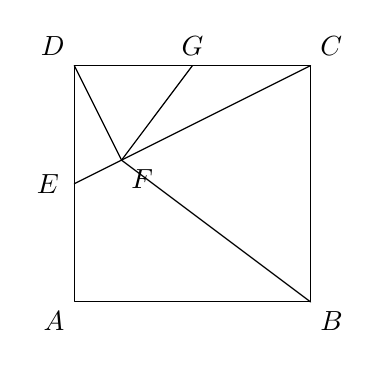
\begin{tikzpicture}[line width=0.45pt, line cap=round, line join=round]
  \coordinate (A) at (0,0);
  \coordinate (B) at (3,0);
  \coordinate (C) at (3,3);
  \coordinate (D) at (0,3);
  \coordinate (E) at (0,1.5);
  \coordinate (G) at (1.5,3);
  \coordinate (F) at (0.6,1.8);

  \draw (A) -- (B) -- (C) -- (D) -- cycle;
  \draw (C) -- (E);
  \draw (D) -- (F);
  \draw (B) -- (F);
  \draw (G) -- (F);

  \node[below left] at (A) {$A$};
  \node[below right] at (B) {$B$};
  \node[above right] at (C) {$C$};
  \node[above left] at (D) {$D$};
  \node[left=2pt] at (E) {$E$};
  \node[above] at (G) {$G$};
  \node[below right] at (F) {$F$};
\end{tikzpicture}
\end{center}
\nopagebreak[4]
   (1) 证明：$B,C,G,F$ 四点共圆；

   (2) 若 $AB=1$，$E$ 为 $DA$ 的中点，求四边形 $BCGF$ 的面积。

\Needspace{4\baselineskip}
\textbf{解析}

\gksubpart{(1)}

\Needspace{5\baselineskip}
设正方形边长为 $s$，取 $D=(0,0)$、$C=(s,0)$、$B=(s,-s)$、$A=(0,-s)$，并令 $DE=DG=t\in(0,s)$。则 $E=(0,-t)$、$G=(t,0)$。直线 $CE$ 的方向向量为 $(s,t)$，而 $DF\perp CE$，由两直线联立可得
\nopagebreak[4]
\[
F=\left(\frac{st^2}{s^2+t^2},-\frac{s^2t}{s^2+t^2}\right).
\]
\Needspace{5\baselineskip}
令 $S=s^2+t^2$、$Q=s^2-st+t^2$，则
\nopagebreak[4]
\[
\overrightarrow{FB}=\left(\frac{s^3}{S},-\frac{sQ}{S}\right),\qquad
\overrightarrow{FG}=\left(\frac{tQ}{S},\frac{s^2t}{S}\right).
\]
两向量点积为 $0$，所以 $BF\perp FG$。又正方形中 $BC\perp CG$，故 $\angle BFG=\angle BCG=90^\circ$，四点 $B,C,G,F$ 共圆。

\gksubpart{(2)}

\Needspace{5\baselineskip}
令正方形边长为 $1$，取 $A=(0,0)$、$D=(0,1)$、$C=(1,1)$、$B=(1,0)$。由 $E$ 为 $DA$ 中点，$G=(\frac12,1)$；作 $DF\perp CE$ 得 $F=(\frac15,\frac35)$。按顶点顺序 $B,C,G,F$ 用鞋带公式：
\nopagebreak[4]
\[
S=\frac12\left|\left(1+1+\frac3{10}\right)
-\left(\frac12+\frac15+\frac35\right)\right|=\frac12.
\]

\gkanswer{答案（1）：\(B,C,G,F\) 四点共圆}

\gkanswer{答案（2）：\(S_{BCGF}=\frac12\)}

\end{answer}
\begin{answer}
\gksolhead{23}{}

\textbf{题目}：

在直角坐标系 $xOy$ 中，圆 $C$ 的方程为 $(x+6)^2+y^2=25$。

   (1) 以坐标原点为极点，$x$ 轴正半轴为极轴建立极坐标系，求圆 $C$ 的极坐标方程；

\Needspace{5\baselineskip}
   (2) 直线 $l$ 的参数方程是
\nopagebreak[4]
   \[
   \begin{cases}
   x=t\cos\alpha,\\
   y=t\sin\alpha,
   \end{cases}\qquad(t\text{ 为参数}),
   \]
   直线 $l$ 与圆 $C$ 交于 $A,B$ 两点，$|AB|=\sqrt{10}$，求 $l$ 的斜率。

\Needspace{4\baselineskip}
\textbf{解析}

\gksubpart{(1)}

\Needspace{5\baselineskip}
代入 $x=\rho\cos\theta$、$y=\rho\sin\theta$ 至圆方程：
\nopagebreak[4]
\[
(\rho\cos\theta+6)^2+\rho^2\sin^2\theta=25,
\]
整理得 $\rho^2+12\rho\cos\theta+11=0$。

\gksubpart{(2)}

\Needspace{5\baselineskip}
参数 $t$ 遍历实数，代入圆方程得到
\nopagebreak[4]
\[
t^2+12t\cos\alpha+11=0.
\]
两根之差的绝对值即弦长，故判别式 $\Delta=|AB|^2=10$。于是
$144\cos^2\alpha-44=10$，得 $\cos^2\alpha=\frac38$、$\tan^2\alpha=\frac53$，所以斜率 $m=\tan\alpha=\pm\frac{\sqrt{15}}3$。

\gkanswer{答案（1）：\(\rho^2+12\rho\cos\theta+11=0\)}

\gkanswer{答案（2）：斜率 \(m=\pm\frac{\sqrt{15}}3\)}

\end{answer}
\begin{answer}
\gksolhead{24}{}

\textbf{题目}：

已知函数 $f(x)=\left|x-\dfrac12\right|+\left|x+\dfrac12\right|$，$M$ 为不等式 $f(x)<2$ 的解集。

   (1) 求 $M$；

   (2) 证明：当 $a,b\in M$ 时，$|a+b|<|1+ab|$。

\Needspace{4\baselineskip}
\textbf{解析}

\gksubpart{(1)}

当 $|x|\le\frac12$ 时 $f(x)=1<2$；当 $|x|>\frac12$ 时 $f(x)=2|x|<2$ 等价于 $|x|<1$。合并得解集 $(-1,1)$。

\gksubpart{(2)}

\Needspace{5\baselineskip}
对 $a,b\in(-1,1)$，有 $(1-a^2)(1-b^2)>0$，而
\nopagebreak[4]
\[
(1+ab)^2-(a+b)^2=(1-a^2)(1-b^2)>0.
\]
又 $1+ab>0$，故 $1+ab>|a+b|$。

\gkanswer{答案（1）：\(M=(-1,1)\)}

\gkanswer{答案（2）：\(|a+b|<|1+ab|\)}

\end{answer}